\documentclass[11pt,letterpaper,english]{article}
\usepackage[T1]{fontenc} % Standard package for selecting font encodings
\usepackage{txfonts} % makes spacing between characters space correctly
\usepackage{xcolor} % Driver-independent color extensions for LaTeX and pdfLaTeX.
\usepackage{hyperref}  %The ability to create hyperlinks within the document
%\usepackage{blindtext} % To create text
%\usepackage{mdwlist} % mdwlist for compact enumeration/list items 
%\usepackage[pagestyles]{titlesec} % related with sections—namely titles, headers and contents
\usepackage{fancyhdr} % header footer placement
\usepackage{float}

\usepackage[top=1in, bottom=1in, left=1in, right=1in] {geometry} % Margins
\usepackage{graphicx}   % Essential for adding images to you document.

\usepackage{sectsty}
\sectionfont{\large}
\subsectionfont{\normalsize}
\subsubsectionfont{\normalsize \it}

\usepackage[font=bf]{caption}% for figure and table captions style
\captionsetup{labelsep=period}

%\setlength{\parskip}{\baselineskip}%
%\setlength{\parindent}{0pt}%


\pagestyle{fancy} % allows you to use the header and footer commands

\raggedright
\begin{document}

\setlength{\parindent}{0in} % Amount of indentation at the first line of a paragraph.

\pagestyle{fancy} \lhead{Revealing the Physics of Galactic Winds with Petascale GPU Simulations} \rhead{Brant Robertson} \renewcommand{%
\headrulewidth}{0.0pt}


\section{PROJECT ACHIEVEMENTS} 

%The project achievements should address the points described below. {\bf This section is typically about 10 pages.} All visual materials, such as charts, graphs, pictures, etc., are included in the page limit; references are {\bf not} included in the page limit. URLs that provide information related to the application should not be included.

``Galactic winds'' are large-scale outflows of mass and momentum from galaxies, and are thought to originate from thermal pressure- or momentum-driven expansion of gas as a result of supernova explosions
from the deaths of massive stars or other star formation-related feedback mechanisms. Almost all modern
theories of galaxy formation invoke galactic winds to regulate the gas content of low-mass galaxies,
keeping them faint and helping us to reconcile the meager abundance of dwarf galaxies relative to the number of low-mass dark matter halos expected from cosmological simulations. 
Understanding galactic winds through simulations is extraordinarily difficult as the
hydrodynamics, radiative cooling, and other physics of the winds must be well-resolved (on $\sim$ few parsec scales) everywhere in the flow that extends kiloparsecs above the galaxy before it merges with the circumgalactic medium. The linear dynamic range is therefore several up to $\sim$ ten thousand, which nominally requires tens of billions of cells over the volume surrounding the galactic disk
to simulate. Since the winds consist of a multiphase medium that includes hot and cold components outflowing at high velocities, capturing all relevant hydrodynamical processes in the wind is best addressed through enormous fixed-grid Eulerian simulation methods.
Our 2017 INCITE project "Revealing the Physics of Galactic Winds with Petascale GPU Simulations" is specifically designed to test the physical mechanisms that launch galactic-scale outflows and shape
their observed properties by leveraging
the unique power of \textit{Titan} and the cutting-edge technology of our GPU-native \textit{Cholla}
code to simulate winds in global simulations of isolated galaxies.
~\\~\\
Semester 1 of our project (Jan-June 2017) resulted in several notable achievements. First and foremost, the project has lead to the single largest hydrodynamic simulation of an isolated galaxy (and asssociated galactic outflow) ever performed to our knowledge. With a volume containing over 17 billion cells, our simulation dwarfs others of this type by over an order of magnitude in computational elements -- a feat uniquely enabled by \textit{Titan}. In order to perform this simulation, the culmination of our work in Semester 1, our project utilized 8192 GPUs on \textit{Titan} for a total of $\sim$8 million core-hours. Our project activities in Semester 1 involved careful preparation for this simulation, including the generation and testing of specialized initial conditions featuring a stable gaseous disk galaxy in hydrostatic equilibrium, an implementation of a supernova feedback scheme to drive a galactic wind, and the improvement of performance,
hydrodynamics algorithms, and other physical modules available in our \textit{Cholla} code. Each of these accomplishments is described in further detail in the sections below. These significant achievements
now position us well to explore and characterize the physics of galactic winds through petascale simulations
on \textit{Titan}, as described in the Project Plans document.

\subsection{Significance of Accomplishments to Date} 

%Explain what advances you accomplished through the INCITE award (impact on community paradigms, valuable insights into or solving a long-standing challenge, etc.). Place the proposed research in the context of competing work in your discipline or business. Reiterate the milestones of your proposal and discuss the accomplishments (planned or unplanned) achieved this year relative to those milestones and allocation use (Section 1aii). Summarize the impact of the results achieved: What conclusions can be drawn, and what is solved because of these results? What new and follow-on investigations have these results motivated?

Our original INCITE proposal focused on the role that radiatively-cooling galactic winds may play in galaxy evolution. While observations routinely show the presence of a fast ($v > 1000$ km/s) yet cool ($T\sim10^4$ K) component of winds being driven out of galaxies with high rates of star formation, numerical simulations of galaxies have thus far failed to reproduce their observed properties. 
Cosmological simulations lack the resolution required to capture correctly the multiphase structure of the winds, and high-resolution simulations of isolated disks have lacked the volume to track gas once it has been driven out of the galaxy. Recent theoretical work (Thompson et al. 2016) has suggested the cold components of the wind originate via radiative cooling
if the wind is sufficiently dense such that its cooling time is shorter than the advection time of the
wind as it leaves the system.
Our project aims to bridge the gap between previous cosmological and isolated disk simulations by producing high resolution simulations of disk galaxies that span a sufficient volume from the wind-generation region within the disk to demonstrate whether starburst-driven winds can cool radiatively and give rise to the 
observed cold wind components.

In order to carry out the simulations described in our proposal, a number of preparatory efforts were completed in the first semester. In Tables 1 and 2, we list the research objectives and milestones from our program's original INCITE proposal. We expand on the current status of each objective and related achievements in the following subsections.
~\\~\\
\begin{table}[h]
%\centering
\vspace{-.12in}
\begin{tabular}{|l|p{5.6in}|} 
\multicolumn{2}{l}{\bf{Table 1: Completed INCITE Proposal Research Objectives}}\\
\hline
\textbf{RO.A} & Simulate galactic outflows with numerical models that allow for supersonic
wind velocities (COMPLETE). \\ \hline
\textbf{RO.B} & Quantify the importance of radiative cooling 
for the multiphase structure of observed galactic outflows (PARTIALLY COMPLETE).\\ \hline
\hline
\end{tabular}
\end{table}


\begin{table}[h]
%\centering
\vspace{-.12in}
\begin{tabular}{|l|p{4.6in}|l|} 
\multicolumn{3}{l}{\bf{Table 2: Completed INCITE Proposal Research Milestones}}\\
\hline
\multicolumn{2}{|l|}{\bf Milestone} & {\bf Objective} \\ \hline
\multicolumn{3}{|c|}{\it Semester 1} \\ \hline
\textbf{RM.A} & Create and test initial conditions for galactic disk simulations ~~~~~~~~~~~~~~~~~~~~ (COMPLETE). & RO.A \\ \hline
\textbf{RM.B} & Implement and calibrate feedback model for driving galactic outflows (COMPLETE). & RO.A\\ \hline
\multicolumn{3}{|c|}{\it Semester 2} \\ \hline
\textbf{RM.C} & Model the multiphase structure and radiative cooling of galactic
outflows on $\sim10$kpc scales (PARTIALLY COMPLETE). & RO.A, RO.B \\ \hline
\multicolumn{3}{|c|}{\it (Originally Planned in) Semester 3} \\ \hline
\textbf{RM.D} & Determine the role of full three-dimensionality on the velocity and density
structure of galactic outflows (PARTIALLY COMPLETE). & RO.A, RO.B\\ \hline
\hline
\end{tabular}
\end{table}

\begin{table}[h]
%\centering
\vspace{-.12in}
\begin{tabular}{|l|p{2.5in}|p{0.7in}|p{0.7in}|p{0.5in}|p{0.7in}|} 
\multicolumn{6}{l}{\bf{Table 3: Completed Research Simulations}}\\
\hline
\multicolumn{2}{|l|}{\bf Simulation Type and Details} & {\bf Objective} & {\bf Resolution} & {\bf Titan Nodes} & {\bf Titan Core Hours} \\ \hline
\multicolumn{6}{|c|}{\it Semester 1} \\ \hline
\textbf{RS.A} & Initial Conditions Test Simulations & RO.A & $N=1024^3$ &512&0.5M\\ \hline
\textbf{RS.B} & Feedback Model Calibration Simulations & RO.A & $N=1024^2\times2048$ &1024&1.5M\\ \hline
\multicolumn{6}{|c|}{\it Semester 2} \\ \hline
\textbf{RS.C} & Adiabatic Wind Simulation & RO.A, RO.B & $N=2048^2\times4096$ &8192&11M\\ \hline
\end{tabular}
\end{table}

%\begin{table}[h]
%\vspace{-.12in}
%\begin{tabular}{|l|l|} 
%\multicolumn{2}{l}{\bf{Table 1: Completed INCITE Proposal Research Objectives}}\\
%\hline
%\textbf{RO.A} & Simulate galactic outflows with numerical models that allow for supersonic
%wind velocities (COMPLETE). \\ \hline
%\textbf{RO.B} & Quantify the importance of radiative cooling 
%for the multiphase structure of observed galactic outflows (PARTIALLY COMPLETE).\\ \hline
%\textbf{RO.C} & Determine the mass and energy coupling of ISM gas to supernova-driven outflows.\\
%\hline
%\end{tabular}
%\end{table}


%\begin{table}[h]
%\vspace{-.12in}
%\begin{tabular}{|l|p{4.6in}|l|} 
%\multicolumn{3}{l}{\bf{Table 2: INCITE Proposal Research Milestones}}\\
%\hline
%\multicolumn{2}{|l|}{\bf Milestone} & {\bf Objective} \\ \hline
%\multicolumn{3}{|c|}{\it Semester 1} \\ \hline
%\textbf{RM.A} & Create and test initial conditions for galactic disk simulations (COMPLETE). & RO.A \\ \hline
%\textbf{RM.B} & Implement and calibrate feedback model for driving galactic outflows (COMPLETE). & RO.A\\ \hline
%\multicolumn{3}{|c|}{\it Semester 2} \\ \hline
%\textbf{RM.C} & Model the multiphase structure and radiative cooling of galactic
%outflows on $\sim10$kpc scales (PARTIALLY COMPLETE). & RO.A, RO.B \\ \hline
%\multicolumn{3}{|c|}{\it Semester 3} \\ \hline
%\textbf{RM.D} & Determine the role of full three-dimensionality on the velocity and density
%structure of galactic outflows (PARTIALLY COMPLETE). & RO.A, RO.B\\ \hline
%\multicolumn{3}{|c|}{\it Semester 4} \\ \hline
%\textbf{RM.E} & Simulate galactic outflows at large dynamic range to generate {\it ab initio} $\sim10$kpc-scale winds from $\sim$pc-scale supernovae bubbles. & RO.A, RO.B, RO.C\\ 
%\hline
%\end{tabular}
%\end{table}

\subsubsection{Research Milestone A: Create and test initial conditions for galactic disk simulations}

A first major accomplishment during Semester 1 of our project is the completion of Research Milestone A: the successful creation of an initial conditions generator for our global galactic disk simulations. The goal of the ICs generator was to 
create realistic gaseous disks with correct dynamical properties set to match real galaxies, while
ensuring numerical stability in simulations with billions of cells.  
In the global disk models we simulate, the dynamics of the model galaxies are set by a background
gravitational potential that consists of a dark matter halo with a Navarro-Frenk-White density profile and
an exponential disk representing the gravitational field generated by the gaseous and stellar components of the galaxy with a Miyamoto-Nagai potential. Given a chosen equation of state for the intestellar gas
in the disk, the equation of hydrostatic equilibrium is solved by balancing the vertical gravitational force from the potential and the vertical pressure gradient generated by the density and pressure profile everywhere in the disk. The gas is initialized to rotate differentially, with the radial velocity
gradient balancing the radial pressure gradient resulting from the surface mass density distribution
of the disk. Outside the disk a spherical hot gaseous halo is added, initialized in 
hydrostatic equilibrium with the
background potential to prevent the external gas from collapsing onto the disk. The initial conditions
generator has been implemented as a module in our code \textit{Cholla}, such that the disk galaxy ICs
can be selected at runtime without re-compiling the code. This feature enables additional flexibility
in testing and validating physics models in idealized simulations before applying them to our global
disk models.
~\\~\\
\begin{figure}[H]
\centering
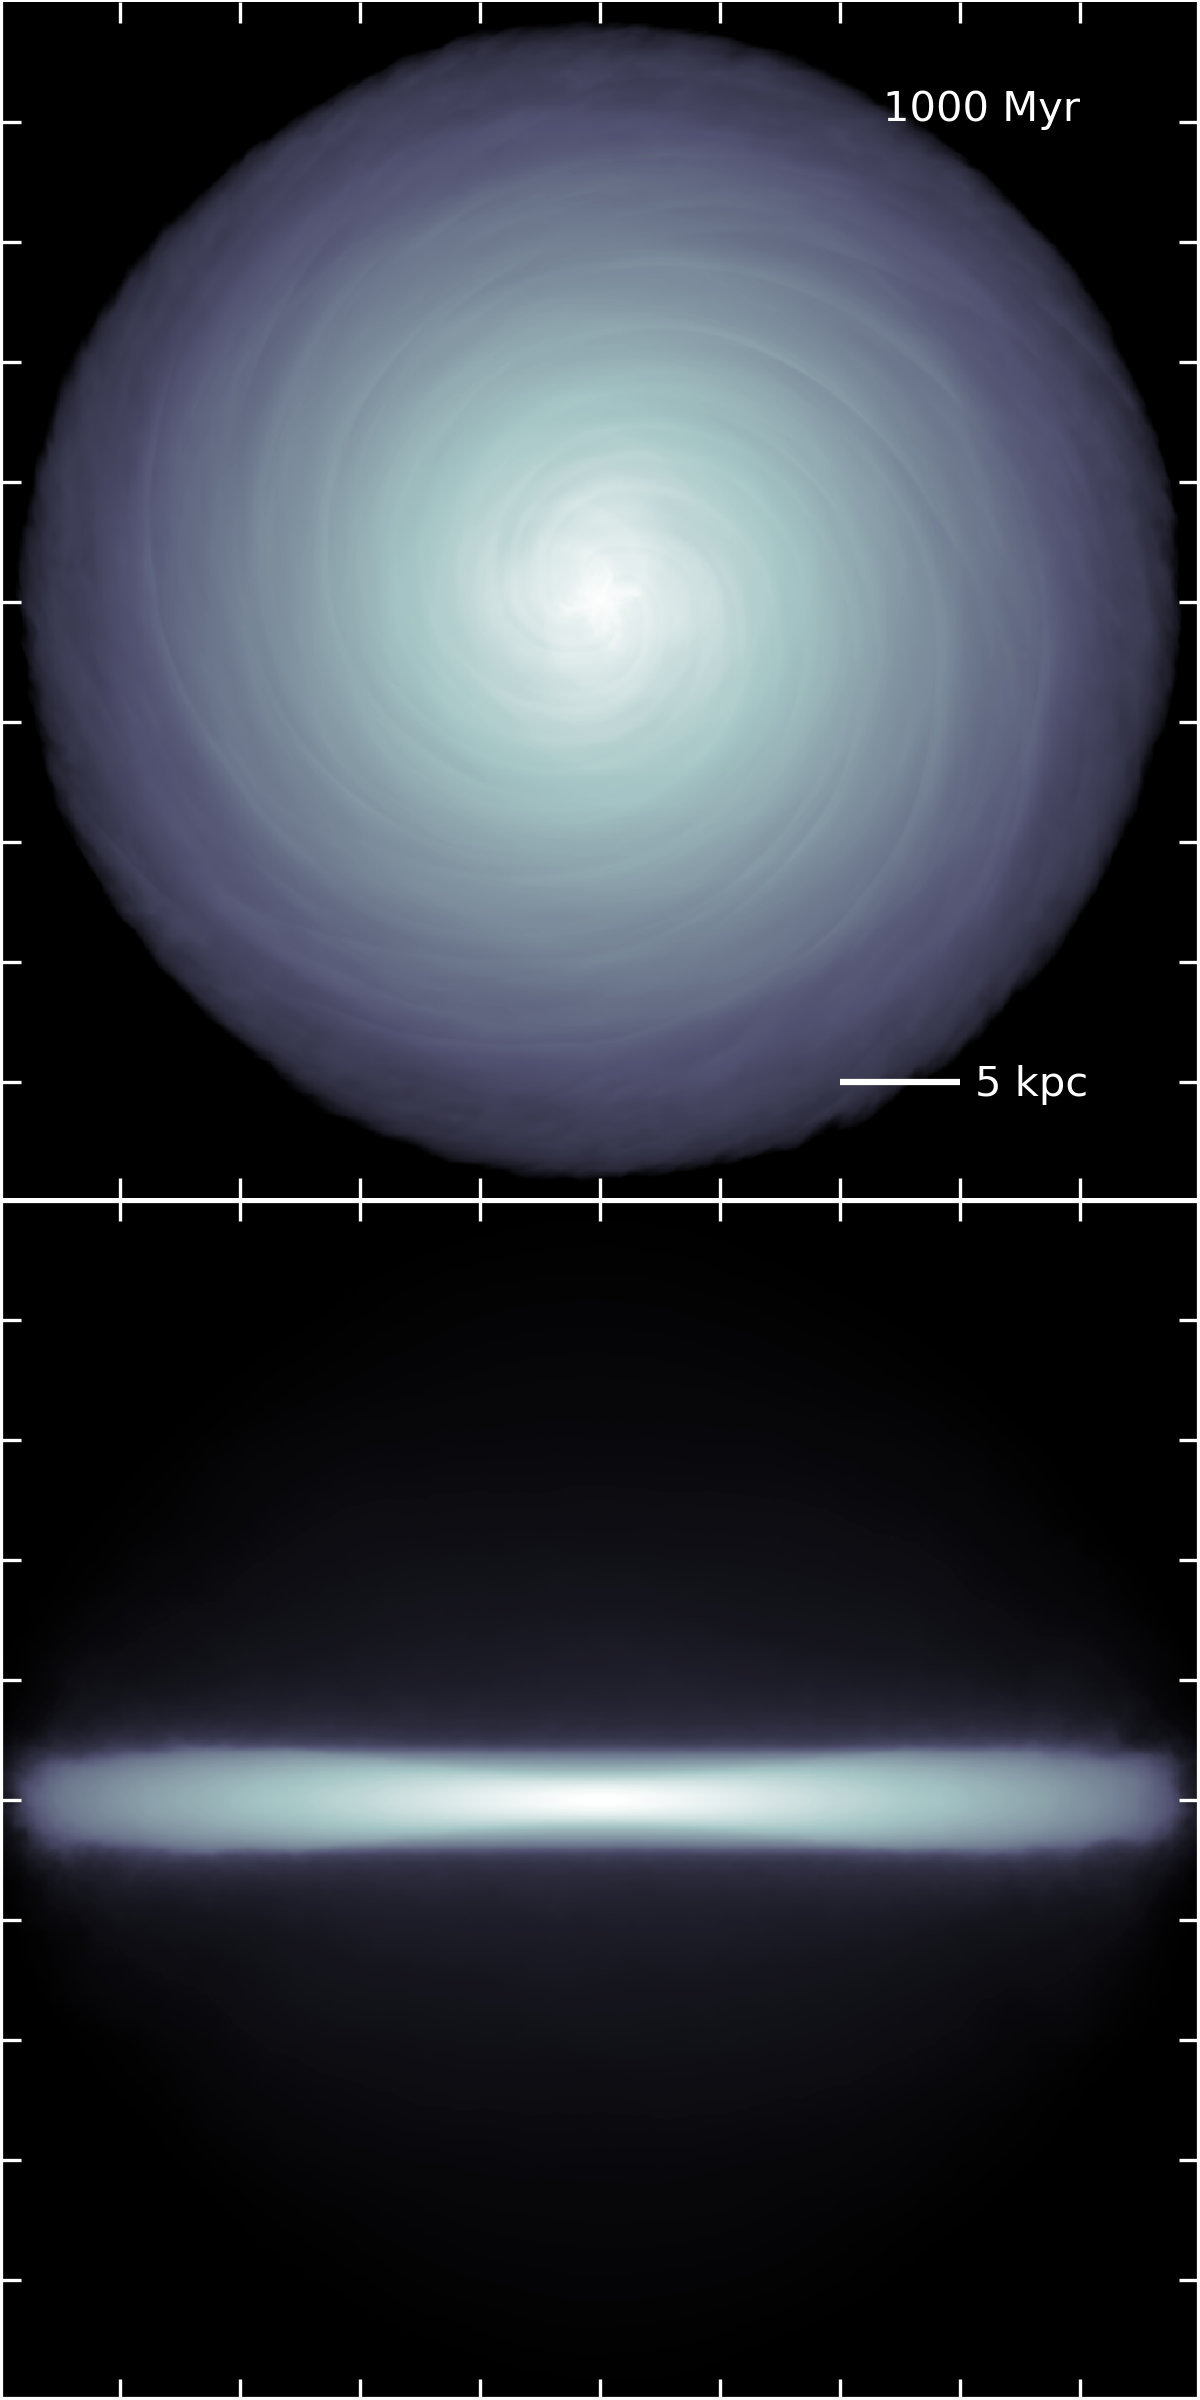
\includegraphics[width=0.35\linewidth]{MW_d.png}
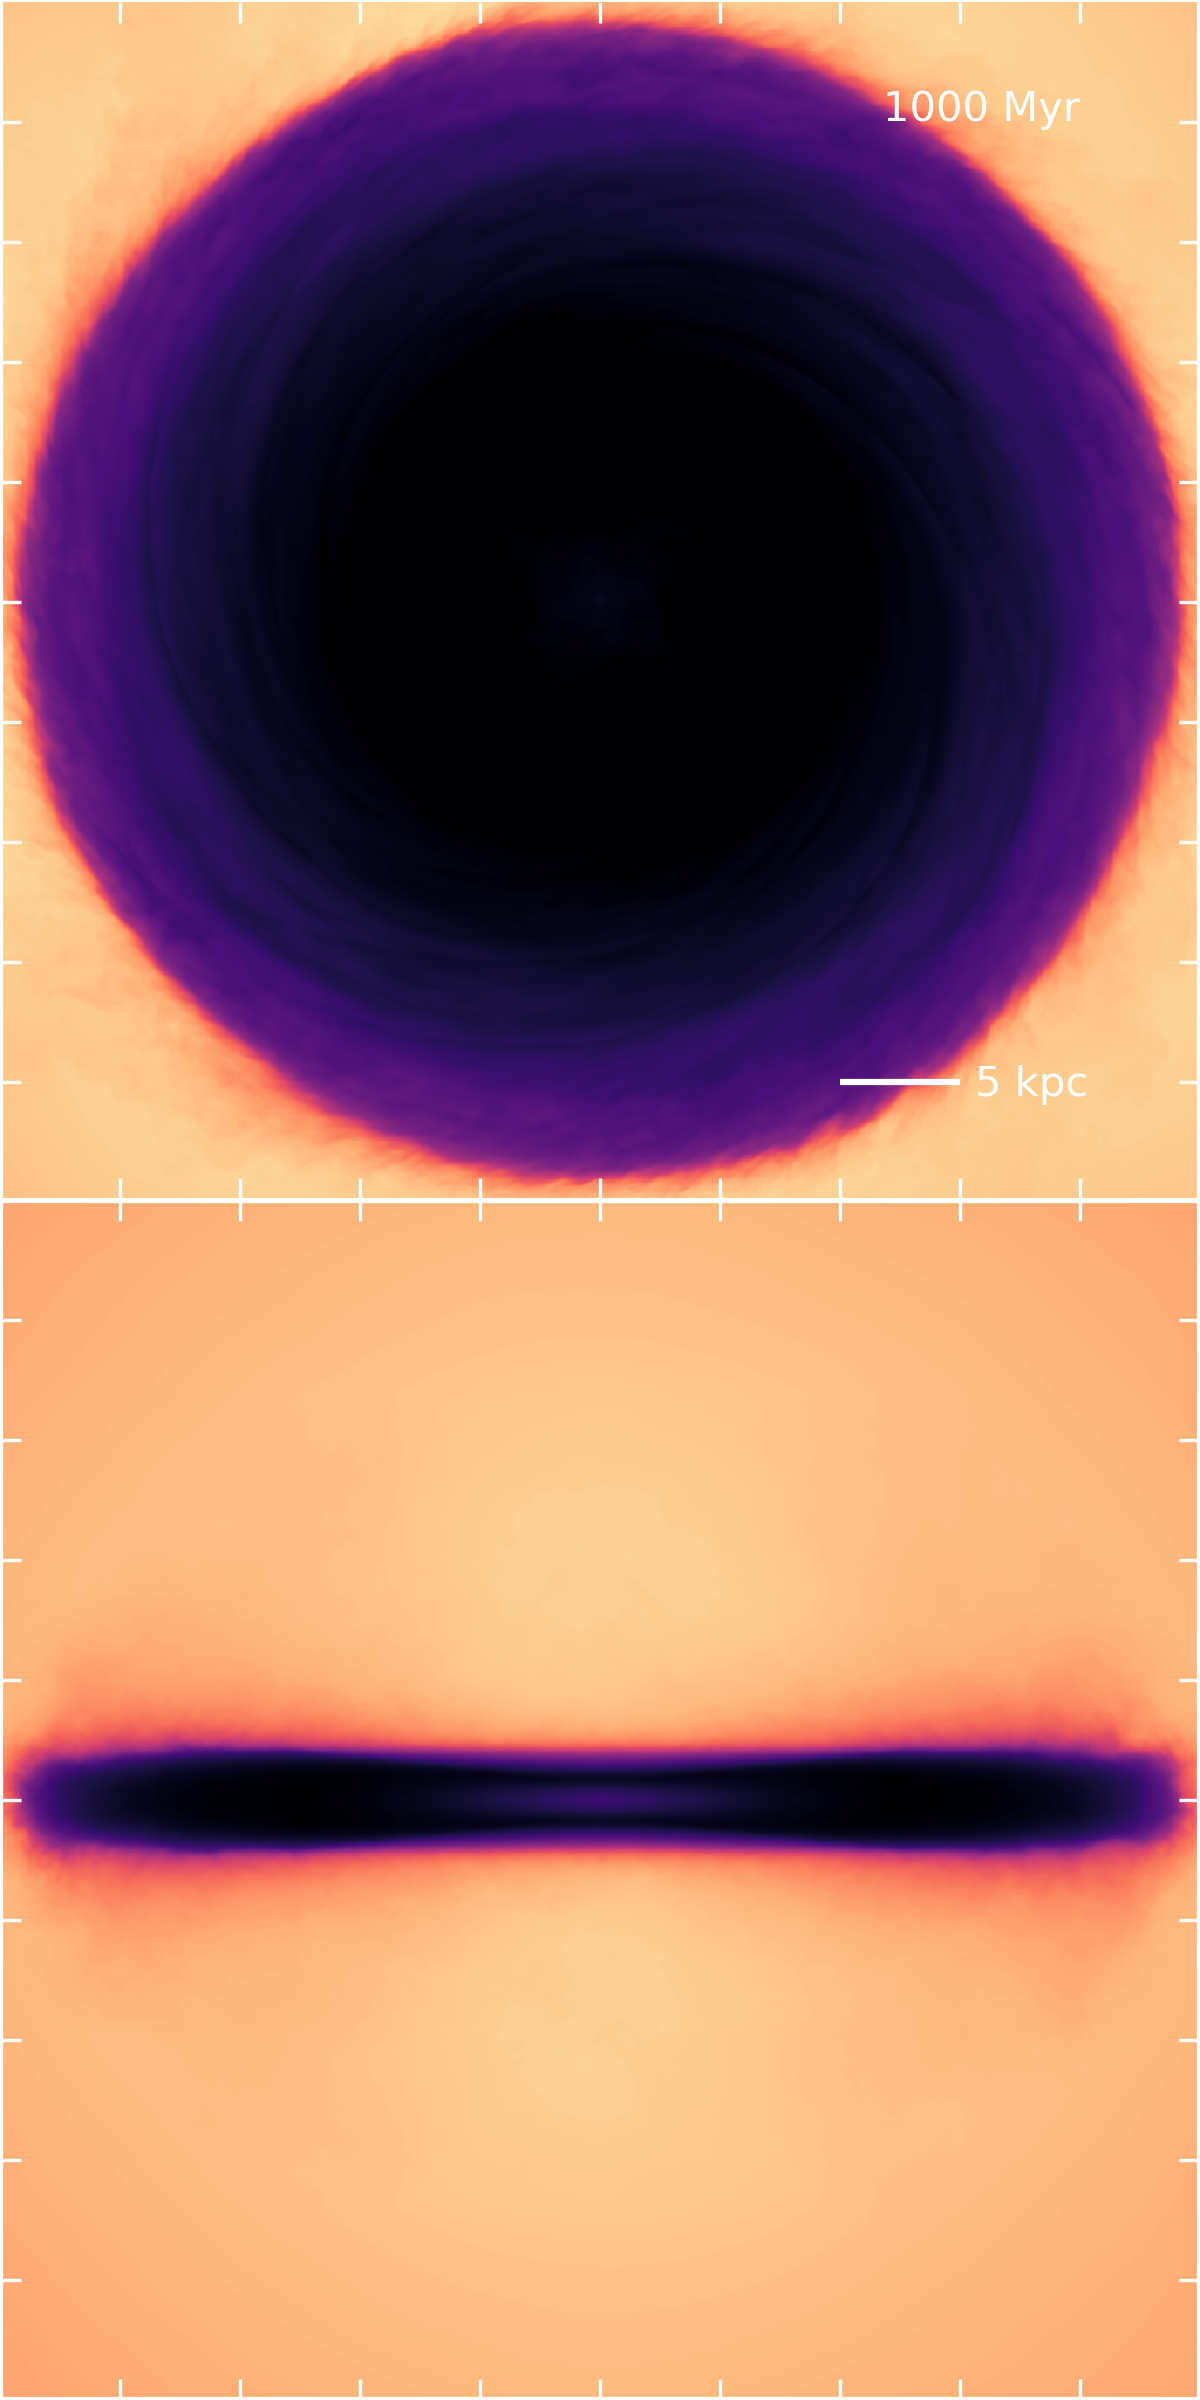
\includegraphics[width=0.35\linewidth]{MW_T.png}
\caption{Isolated Milky Way-like disk galaxy after 1 Gyr of evolution, simulated with
1024$^3$ cells. Shown are the density (left) and temperature (right) projected
in the x-y (upper) and x-z (lower) planes. The model includes a background gravitational
potential for the dark matter halo and disk, a gaseous disk with an exponential surface
mass density profile, and a hot gaseous halo in hydrostatic equilibrium. To test for
the thermal and dynamical stability of the initial conditions, the wind driving mechanisms
have been turned off. The galaxy is very stable over billion year timescales, more than sufficient for simulations
of the launching of galactic-scale winds. The simulated evolution of a smaller, M82-like galaxy
shows comparable excellent performance. These initial conditions complete Research Milestone A listed in Table 1.}
\label{fig:MW_ICs}
\end{figure}

We have used the initial conditions generator to create two carefully crafted galaxy models representing
a Milky Way-like galaxy and a mimic of the nearby starburst galaxy M82 with a well-studied galactic wind.
To test for thermal and dynamical stability, we have performed calibration simulations that
evolve these galaxy models for many rotational periods in isolation and without including
an engine for driving galactic winds. 
A snapshot of the Milky Way model after 1 Gyr of evolution is shown in Figure \ref{fig:MW_ICs}. The left panels show projected gas density in the x-y and x-z planes, while the right panels show projected gas temperature. After many millions of years of evolution, the differential rotation of the gas in the disk leads to the minor spiral features that can be seen in the x-y density projection. A small amount of turbulence is generated on the surface of the disk due to the shear between disk and halo gas (only the disk gas is given an initial rotation). Otherwise, the disk and halo look almost identical to their initial setup and validate the physical realism of the initial conditions generator.
Adiabatic simulations of the Milky Way and M82 initial conditions have demonstrated that they are both stable for at least a gigayear, far longer than the duration of our galactic wind simulations. Compared to similar projects in the literature, our initial conditions are considerably more realistic (see e.g. Cooper et al. 2008, Fielding et al. 2017). Most models simply use an isothermal disk with no halo gas, or an isothermal gaseous 
halo out of hydrostatic equilibrium -- we have verified in experimental calculations that
simple isothermal halos lead to unphysical accretion onto the central disk, and that capturing the effects
of halo gas swept by the wind requires physically realistic galaxy models like what we employ. We view these
initial conditions as a significant advancement in the physical realism of isolated galaxy models and the
developmental work conducted through this program necessary for ensuring numerically stable galaxy
models in simulations using many billions of cells.

\subsubsection{Research Milestone B: Implement and calibrate feedback model for driving galactic outflows}

A second major accomplishment of our program is the completion of Research Milestone B: an original
implementation of a supernova feedback model that will allow us to test the premise that supernova-driven winds can cool radiatively at large radii from the disk. The theoretical framework for modeling
galactic winds analytically harkens to Chevalier \& Clegg (1985; CC85), who computed the radial density, velocity,
and temperature profiles of a centrally-driven outflow in spherical symmetry. In CC85, the supernova
feedback from the deaths of massive stars leads to an input of mass and energy at the center of the
galaxy in a ``gain region'', resulting in a spherically-expanding flow of gas that
eventually accelerates to a supersonic wind velocity. The CC85 model considers neither 
the potential 
radiative cooling of the wind nor the effect of a gravitational potential on the outflow dynamics (physics
we include in our simulations).
Despite the simplicity of the CC85 model, X-ray observations indicate that the model provides a good fit for the central region of the superwind in M82 (Strickland \& Heckman, 2009). More recent models have extended the CC85 model to include the effects of both gravity and radiative cooling (Wang 1995, Thompson 2016). These models suggest that given sufficient mass-loading of the hot wind, dramatic cooling can take place at radii 1 - 10 kpc from the wind-generation radius, which could account for the fast-moving, cool gas observed around starburst galaxies. The simulation of galactic-scale winds that led to the \textit{ab initio} formation of radiatively
cooling outflows would represent a signficant scientific result in astrophysics, and serves as strong
motivation for the prior and continuing work of our INCITE program.
~\\~\\
In order to test effectively this picture for the physical origin of cold multiphase material in galactic
winds, we have created a supernova feedback model that matches the CC85 model as closely as possible. 
Our current feedback model assumes a constant rate of mass and energy injection within a starburst radius
of the gain region, with the mass and energy injection set by three parameters: the star formation rate, the mass-loading factor, and the supernova thermalization efficiency. Our initial models use consistent
values for the past star formation rate, mass-loading, and supernova thermalization efficiency as inferred from observations of M82. The resulting wind can then be compared against the theoretically-calculated model, as shown in Figure \ref{fig:CC85}. 
~\\~\\
Our fiducial feedback model used in the simulations of an M82-like galaxy uses a star formation rate of 
20 $M_\odot$/yr, a mass-loading factor of $\beta_\mathrm{hot} = 1.4$ (the ratio of the mass in the hot wind to the
mass expelled from supernovae into the interstellar medium), and a supernova thermalization efficiency of 
$\alpha = 0.9$ (describing the fraction of supernovae energy thermalized into the internal energy of interstellar medium gas). Figure \ref{fig:CC85} displays the density, velocity, temperature, and pressure of the resulting wind as a function of radius. Plotted in Figure \ref{fig:CC85} are both the exact CC85 solution (black line), as well as the fluid properties measured along the $z$-axis of one of our galactic-scale outflow calibration simulations after 5 (blue), 15 (orange), and 25 Myr (green). In these simulations, we initialize the supernova feedback after 5 Myr, and the outflow quickly evolves from the initial conditions reflecting the structure of the gaseous disk and halo (blue line) to radial profiles
at 15 and 25 Myr (shown as the orange and green lines) that match the CC85 solution (black) extremely
closely. Indeed, the evolved models in Figure \ref{fig:CC85} are difficult to see because they lie \textit{directly} in agreement with the exact solution, demonstrating that within 10 million years, this feedback model has set up a stable wind with outflow parameters that match those expected from CC85 (note that this is a simulation \textit{without} radiative cooling). Our results represent achievements both for the CC85 analytic model and our code \textit{Cholla}, and complete Research Milestone B.
In Year 2, we will continue our on-going developmental work to extend our feedback model to incorporate more realistic versions of supernova feedback (see Project Plan).

\begin{figure}[H]
\centering
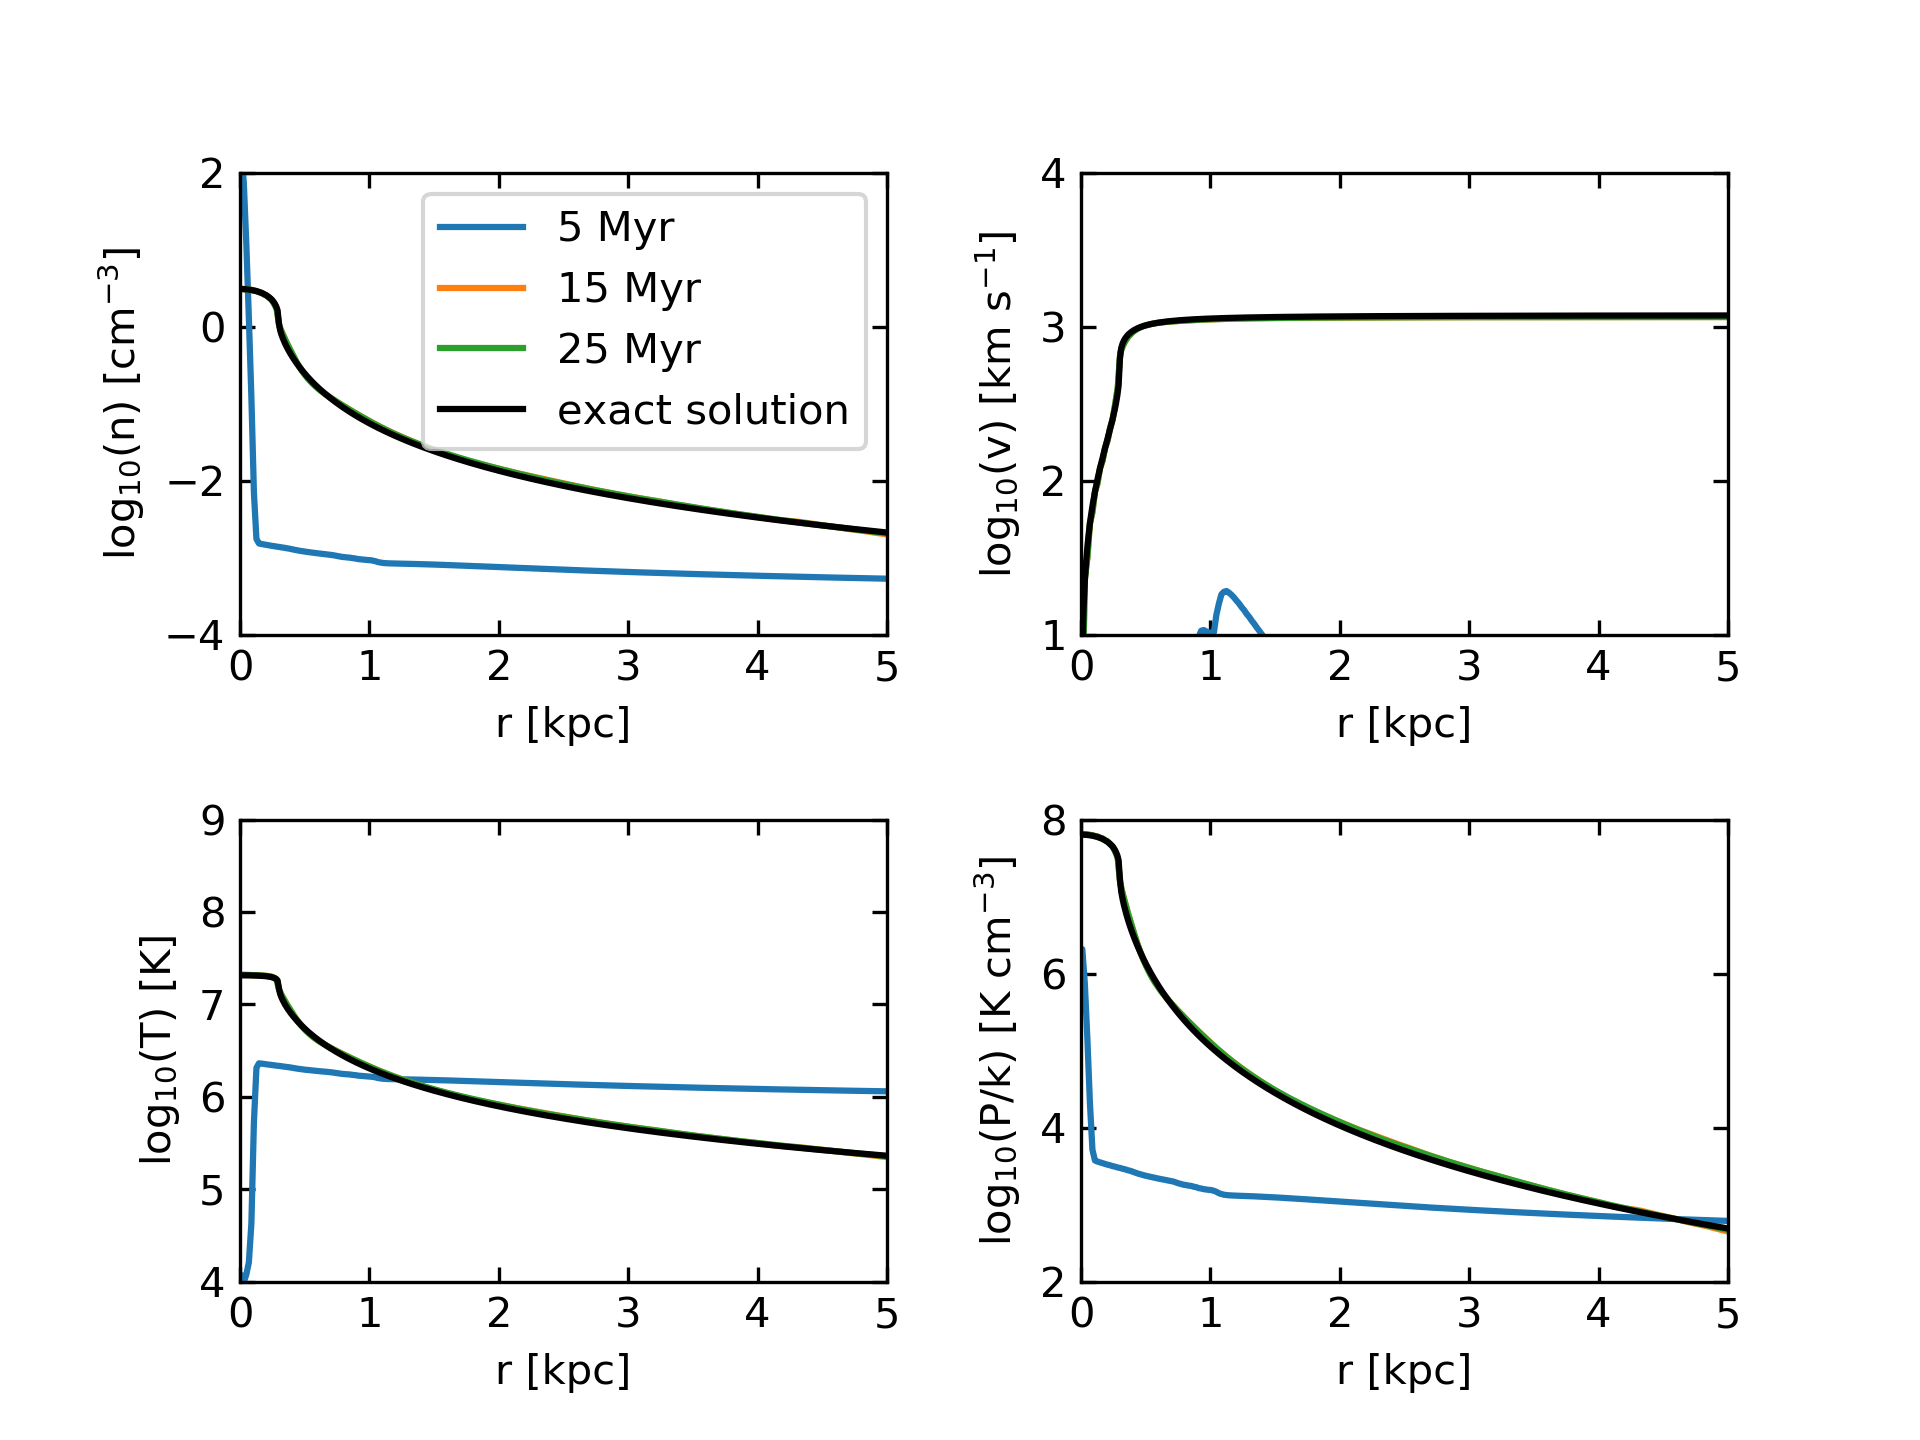
\includegraphics[width=0.8\linewidth]{CC85.png}
\caption{Radial density (upper left), velocity (upper right), temperature (lower left), and pressure (lower right profiles) of the analytical Chevalier \& Clegg (1985; CC85) model for the M82 galactic wind, and values measured from our 512x512x1024 test simulation with the \textit{Cholla} code (colored lines). 
Although the initial conditions of the simulation start far away from the CC85 model (blue lines), the
outflow properties quickly converge to the CC85 solution and maintain the solution over
15 (orange) and 25 (green) Myr timescales.}
\label{fig:CC85}
\end{figure}

~\\
As a control for our radiatively-cooling wind simulations, we have run a production-scale adiabatic simulation with our fiducial feedback model parameters. Our production simulations are run on grids with $2048\times2048\times4096$ cells, in a domain with dimensions 5 kpc $\times$ 5 kpc $\times$ 10 kpc, giving a resolution of $\Delta x=4.9$ pc at all locations in the simulation volume. Density and temperature projections for this adiabatic control simulation after 30 million years of evolution are shown in Figure \ref{fig:adiabatic_2048}. The biconical outflow driven by the central energy and mass input is clearly visible in the temperature projection, as is the fall-off in temperature with radius due to the expansion of the flow. The energy injection has resulted in the blow-out of all of the gas from the central region of the disk. This simulation represents by far the largest hydrodynamic simulation of an isolated galaxy ever performed, and its number of computational elements tops that of even large cosmological simulations (e.g. the IllustrisTNG simulation, see Nelson et al. 2017, which has $\sim$15.6 billion hydrodynamic particles, vs. our $\gtrsim$17 billion cells). Thus, despite the fact that this calculation is merely our control simulation, it represents a major achievement and technological milestone for our program.
An advantage of our current simple feedback scheme is that it allows us to easily adjust the three feedback model parameters (star formation rate, mass-loading, and thermalization efficiency) to determine what range of parameters lead to galactic outflows that can cool on large scales. With our remaining 2017 allocation, we will be able to perform three production simulations with radiatively cooling physics that will explore the range of necessary mass-loading in order to enable the development of cold multiphase components in the
galactic-scale outflows (see Project Plan for details).

\subsubsection{Research Objective A: Simulate galactic outflows with numerical models that allow for supersonic wind velocities}

With the completion of Research Milestones A and B in Semester 1, we have achieved Research Objective A of our INCITE program: to simulate galactic outflows with numerical models that allow for supersonic wind velocities. While theoretical models had indicated that these starburst-driven winds should achieve supersonic velocities, the planar geometries employed in previous studies prevented winds from developing a sonic point (see discussion in Martizzi et al. 2016). By simulating winds on a global scale that allow
for the outflows to diverge geometrically and develop a sonic point, we have demonstrated that winds achieve supersonic velocities and that in scenarios where the injection rates can be well-approximated by the CC85 model the large-scale features of those winds can be well-approximated by the analytical CC85 theory. We now turn to a discussion of the radiatively-cooling wind models that are the focus of our research program.



\subsubsection{Research Milestone C: Model the multiphase structure and radiative cooling of galactic outflows on $\sim$10 kpc scales}

Our 2016 INCITE proposal devoted Semester 2 to achieving Research Milestone C. As we are only a few weeks into Semester 2, we do not yet have most of the results, but we do have some early indications that the predictions of the theoretical models with radiative cooling will be born out in our production simulations. Figure \ref{fig:cooling_sim} shows the temperature in slices through the x-z plane for a calibration simulation (resolution $512\times512\times1024$ cells) with and without radiative cooling (left and right, respectively). Both snapshots show the simulations after 22 million years of evolution. While the cold gaseous disk is clearly visible on both simulations, the simulation with cooling also shows a large amount of gas between 2 - 5 kpc that has cooled to $10^4$ K where the physical cooling mechanisms
become inefficient. Early analysis of this simulation suggests that the velocities of this cool gas may be consistent with observations, which would make these the first simulations to reproduce successfully gas in this phase in large-scale galactic winds. The exciting indications of successful
radiatively cooling wind simulations motivate the remainder of our calendar year 2017 work, and the renewal of the
progam into 2018 as outlined in the Project Plan document.


\begin{figure}[H]
\centering
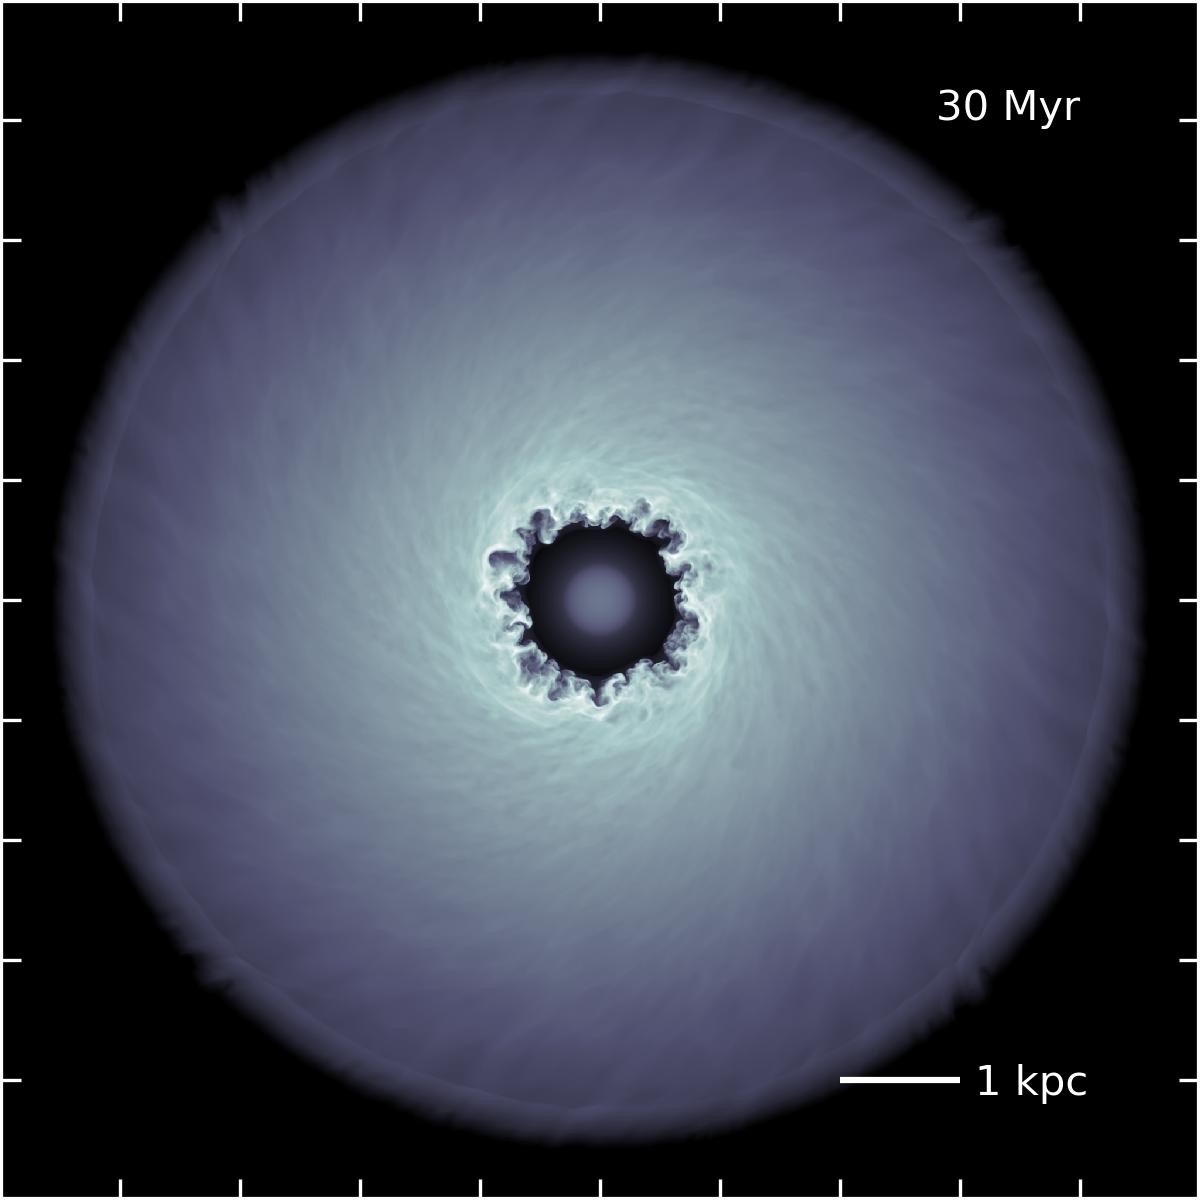
\includegraphics[width=0.35\linewidth]{M82_dxy.png}
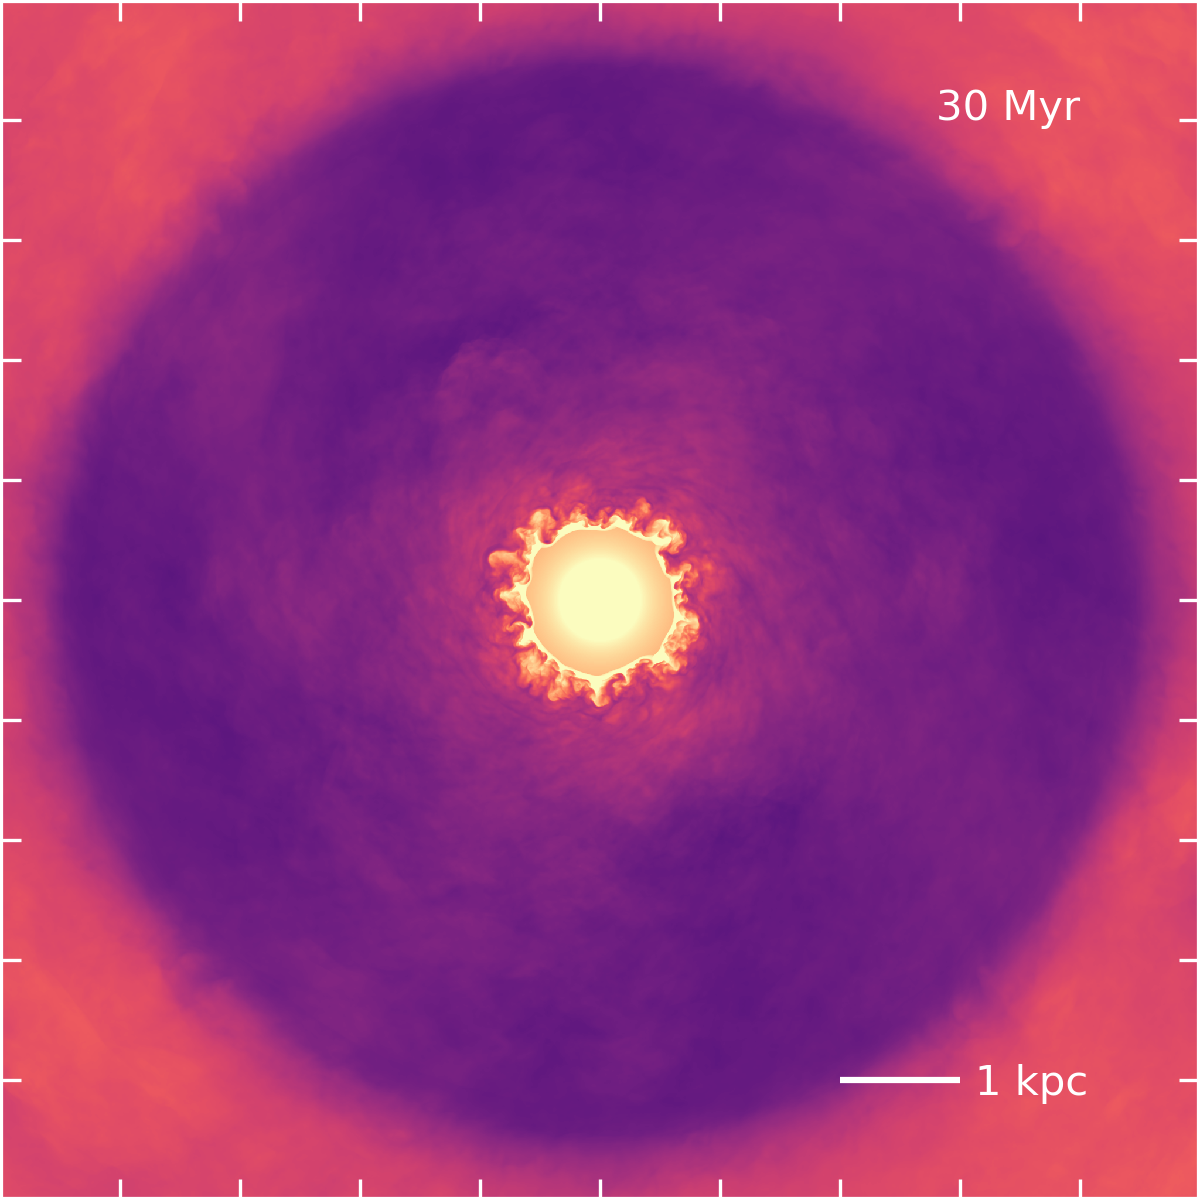
\includegraphics[width=0.35\linewidth]{M82_Txy.png}
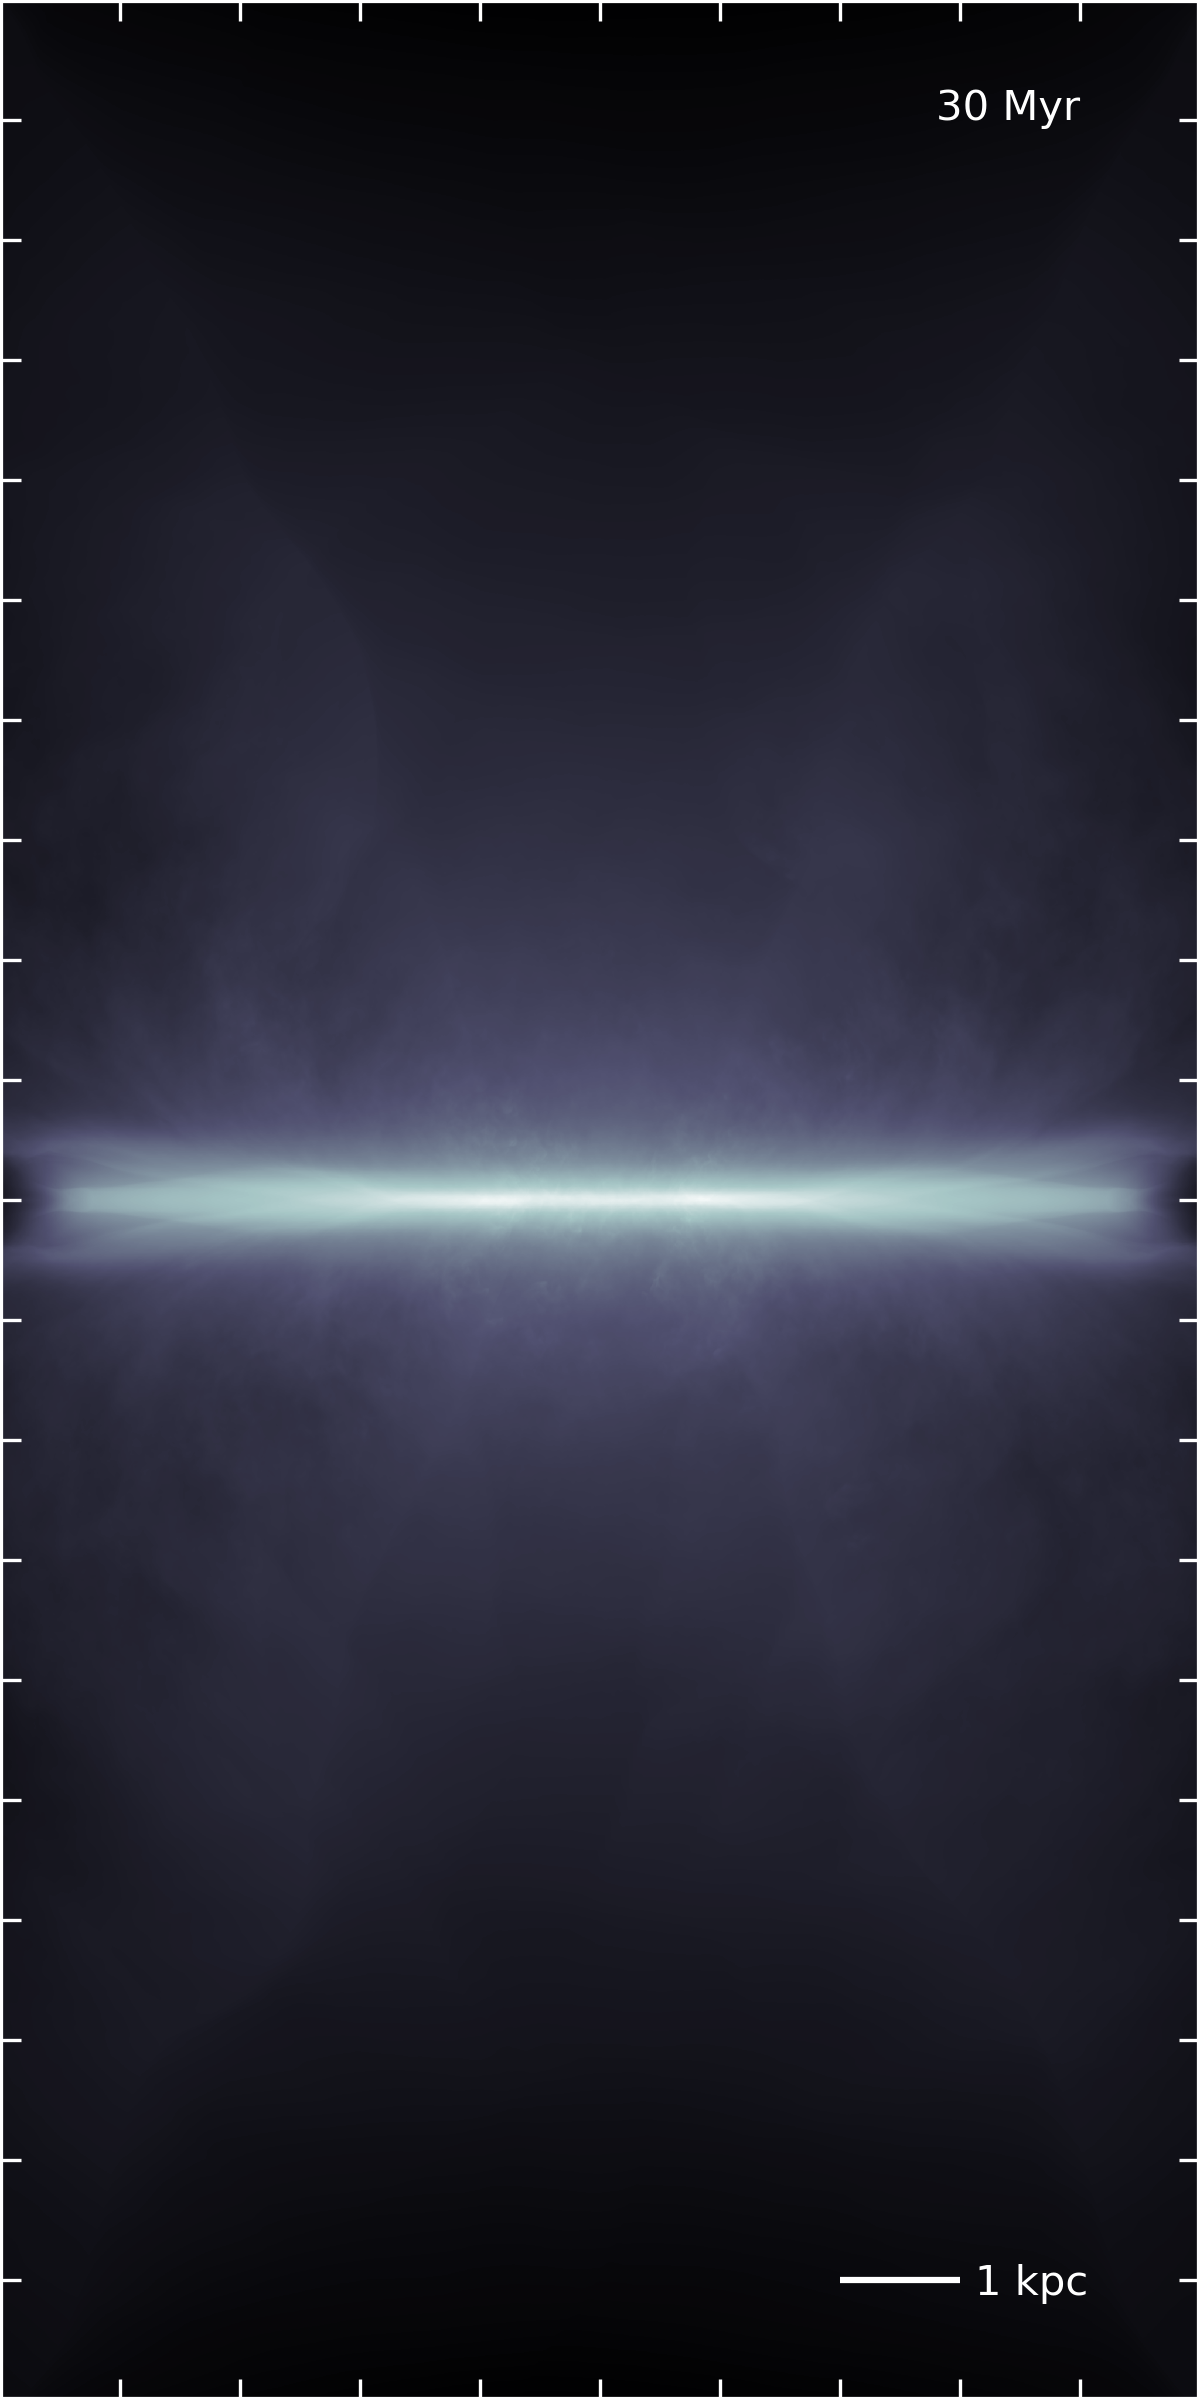
\includegraphics[width=0.35\linewidth]{M82_dxz.png}
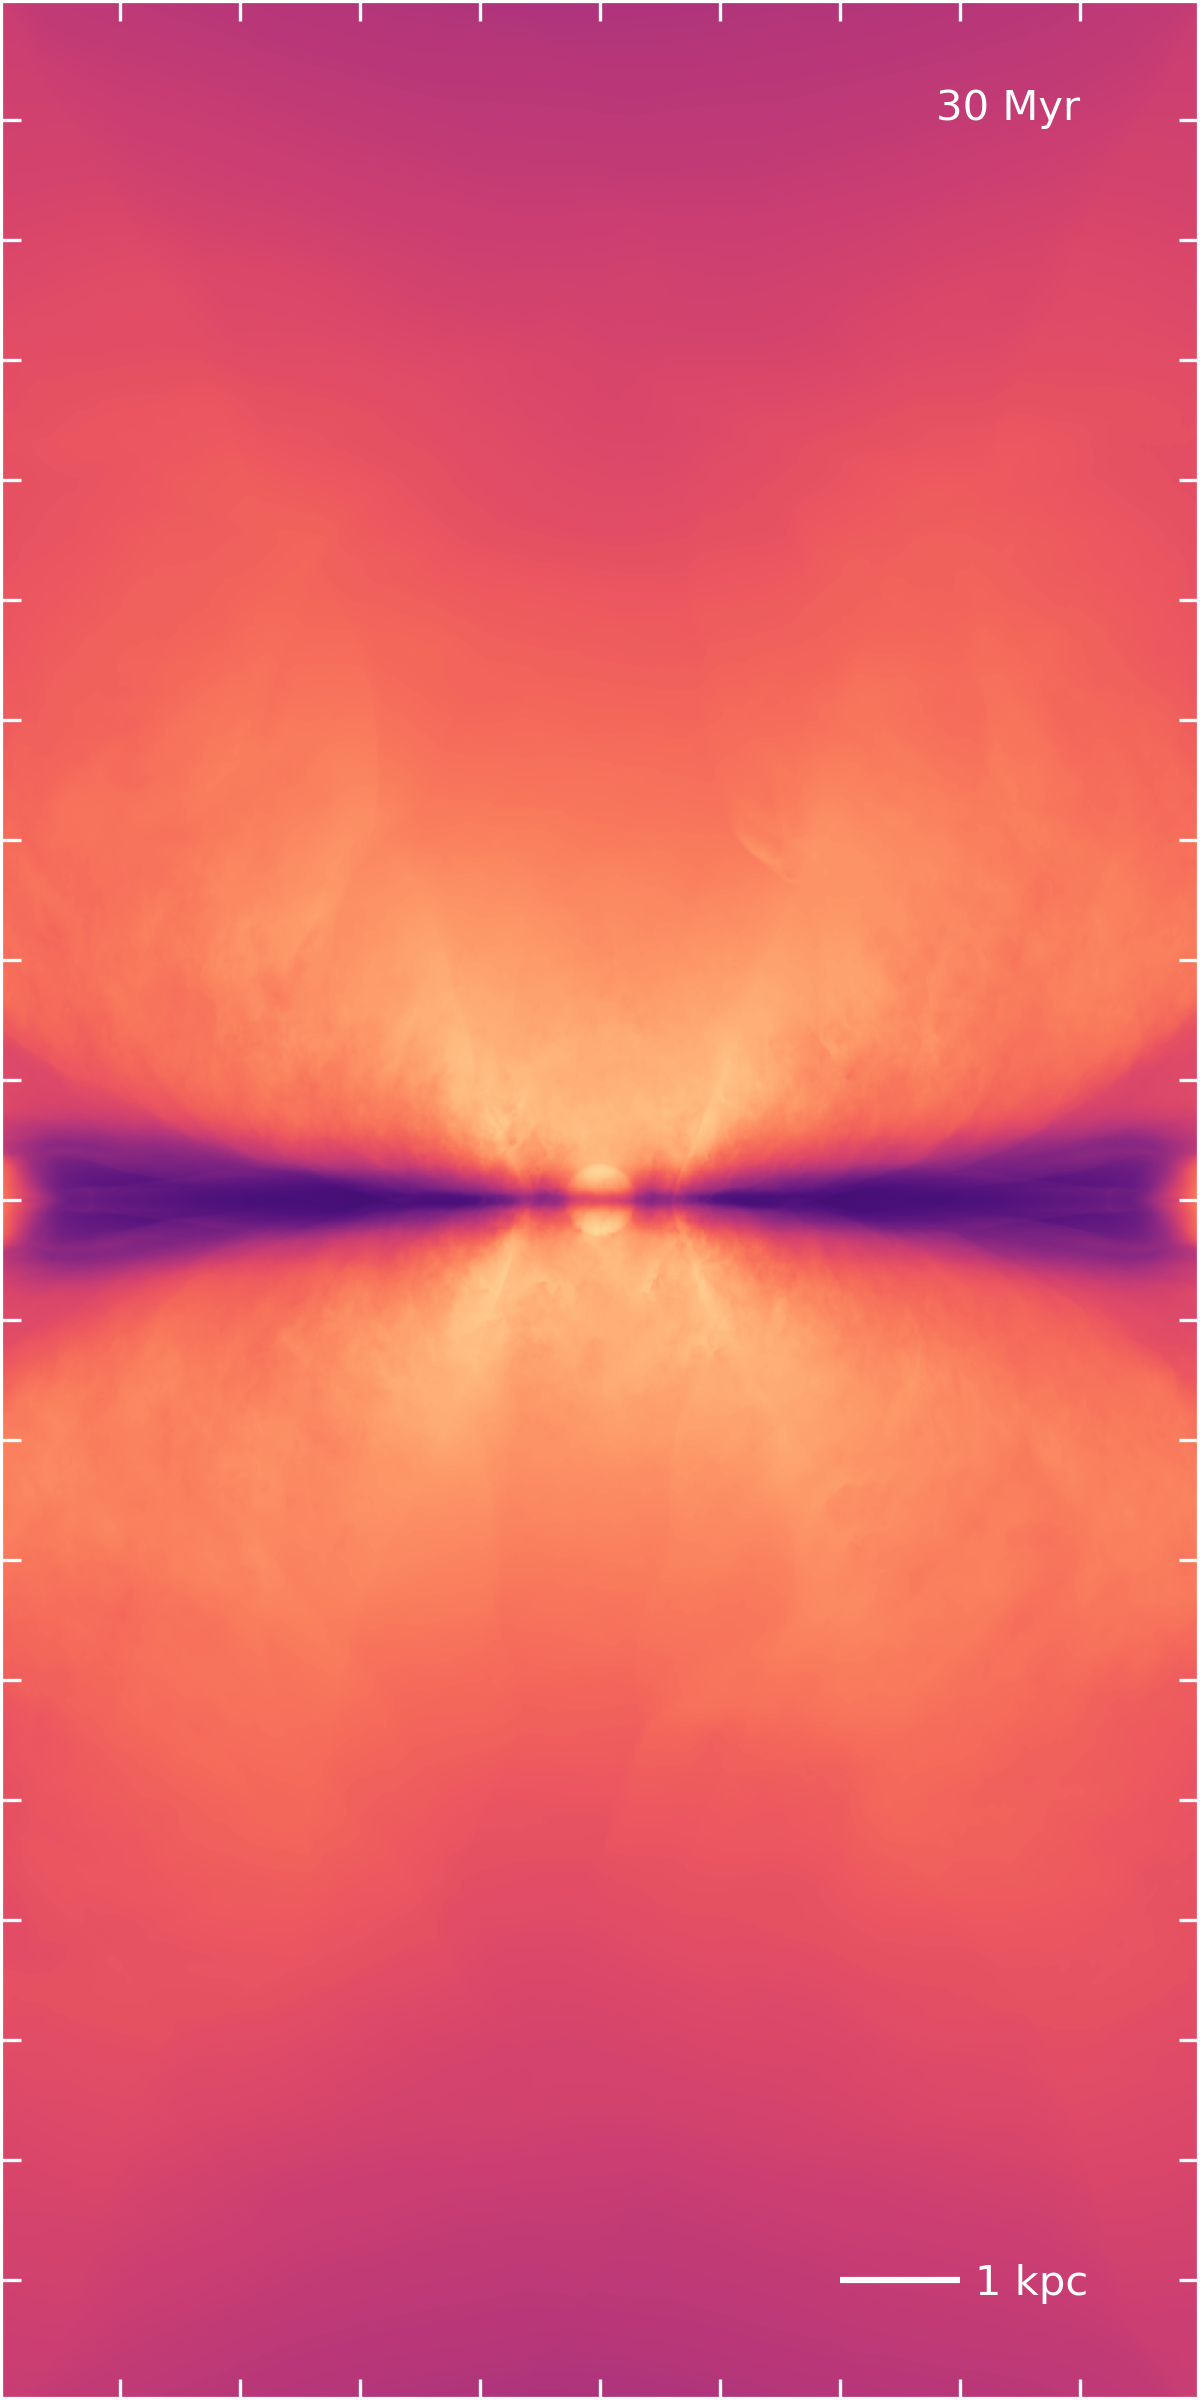
\includegraphics[width=0.35\linewidth]{M82_Txz.png}
\caption{Global disk simulations of an M82-like galaxy at high resolution (2048x2048x4096 cells) using adiabatic gas physics, the largest simulation of an isolated disk galaxy ever performed (to our knowledge). Shown are
the density (left) and temperature (right) projections in the x-y (upper) and x-z (lower) planes. The gas temperatures range from $10^{4}$K (purple) in the cool disk to $10^7$K in the hot outflow (peach). The simulations include a model for injecting mass and energy associated with supernovae feedback at the center
of the system, driving a large-scale galactic outflow.
By performing a global simulation the three-dimensional nature of the wind is captured, allowing the wind to
develop a sonic point and become a supersonic flow outside of the disk. The outflow precisely matches the
wind structure of the Chevalier and Clegg (1985) analytical model (as demonstrated in the  Figure \ref{fig:CC85} above) that reproduces the bulk properties of the galactic outflow in M82.}
\label{fig:adiabatic_2048}
\end{figure}

\begin{figure}[h]
\centering
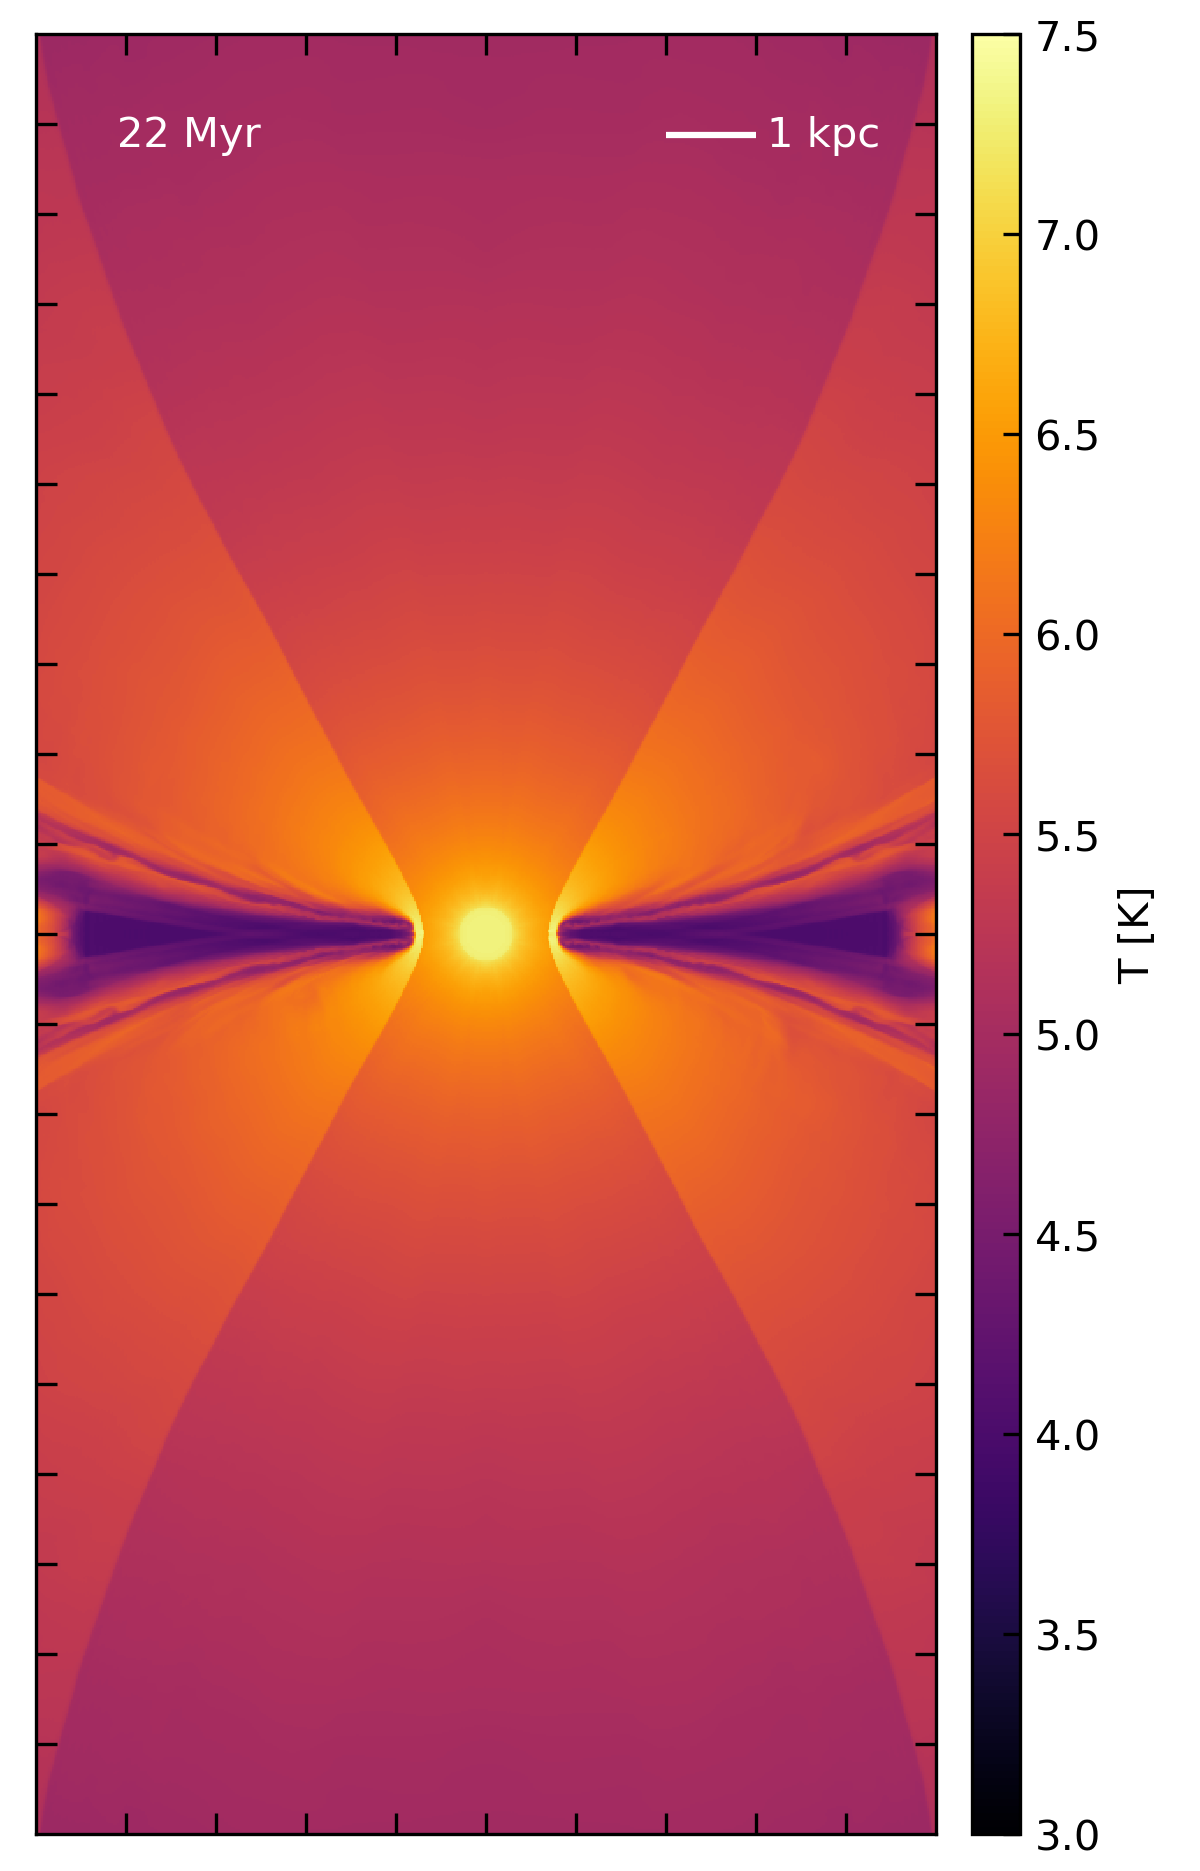
\includegraphics[width=0.35\linewidth]{Tslice_nocool.png}
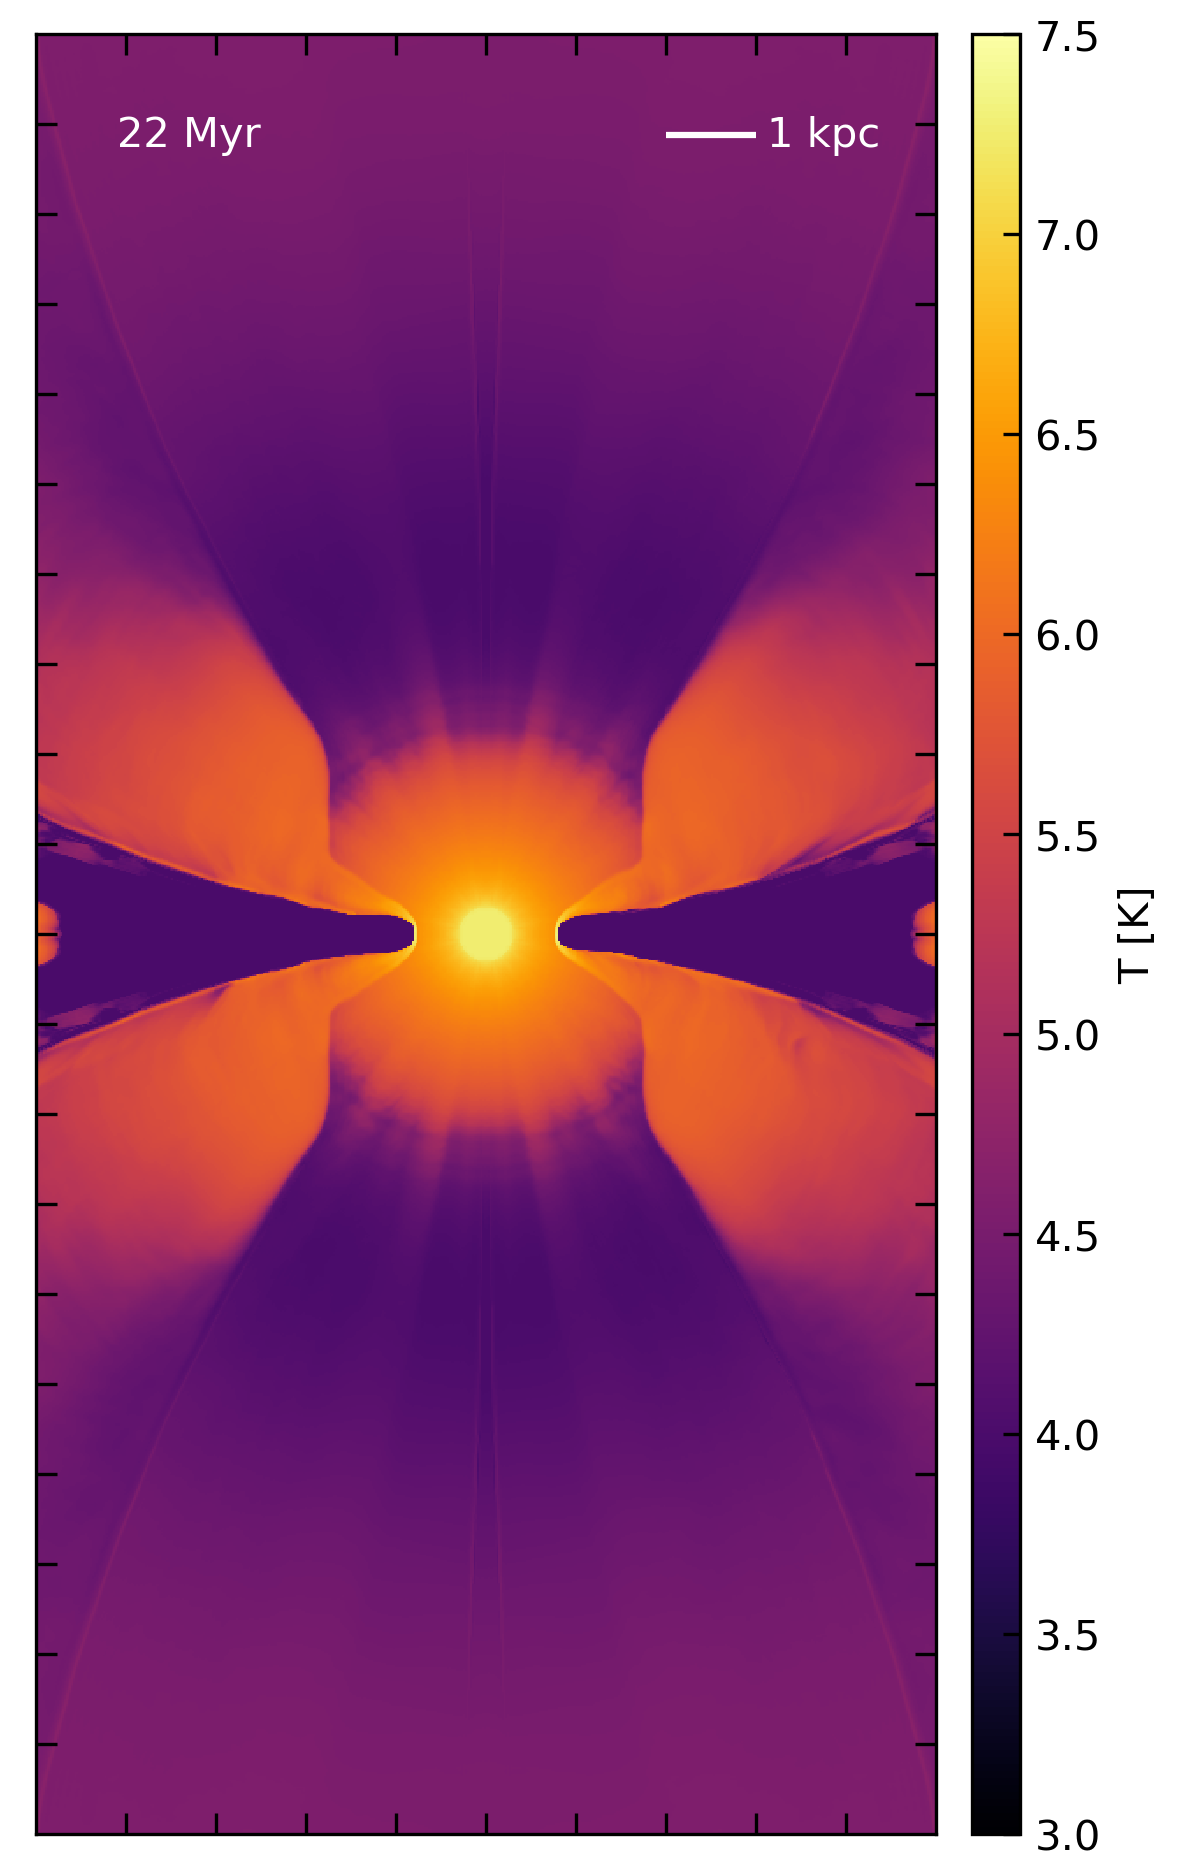
\includegraphics[width=0.35\linewidth]{Tslice_cool.png}
\caption{Initial results from global disk simulations, comparing adiabatic (left) and radiatively-cooling (right) gas. Shown are temperature slices of the x-z plane at y=0 for a 512x512x1024 simulation of an M82-like galactic outflow. Given the supernova feedback parameters assumed, the Thompson et al. (2016) analytical wind model would predict that the galactic outflow should cool radiatively on a timescale shorter than the wind advection timescale across the simulation volume. Indeed, when radiative cooling is included, the outflow cools and demonstrates that the Thompson et al. (2016) explanation for the origin of cold absorbers in galactic outflows is plausible. With this important demonstration achieved, our program will now perform these simulations at higher resolution and with more realistic supernovae feedback modeling.}
\label{fig:cooling_sim}
\end{figure}

~\\~\\
We are currently finalizing the feedback model parameters for our production-scale radiative cooling wind simulations. Once we have decided on the appropriate physical parameters, 
we will run three production simulations with radiative cooling that will be compared with the adiabatic simulation presented in the previous section and thereby allow us to definitively answer the question posed by our Research Objective B: Quantify the importance of radiative cooling for the multiphase structure of observed galactic outflows. These production simulations will exhaust the remainder of our 2017 core-hour
allocation, and set the stage for our work in 2018.
\subsection{Allocation Use} 

%Summarize your project's allocation use to date this year: percent of allocated core-hours used on each platform, job size distribution, number of users, etc. Associate the resource use with particular results where possible. Also summarize your project's projected use from now until the end of December (i.e., end of current allocation year): anticipated percent of allocated core-hours used on each platform, job size distribution, etc. Associate this resource usage with anticipated results. Do you expect your usage to be evenly distributed throughout the remainder of this year? If not, explain.
As of July 25th, our project has used 8.14 million core-hours, of the 46 million core-hours we were allotted for Year 1. This burn rate follows closely the original plans in our 2016 INCITE proposal, and we have been
able to reprioritize and reach production simulation capability more quickly than first planned. In particular, our calibration simulations were more efficient than initially anticipated, which resulted in our usage for Semester 1 totaling $\sim1.5$ million hours, rather than the 5 million we projected in the proposal. The large calibration simulations consisted of two $1024^3$ simulations, each run on 512 GPUs, and a $1024\times1024\times2048$ simulation run on 1024 GPUs. The first two were tests of the stable Milky Way and M82 initial conditions (such as the simulation shown in Figure \ref{fig:MW_ICs}). The third, larger calibration simulation was a test of the supernova feedback model and wind generation scheme for the adiabatic model. The initial conditions test simulations took only $\sim$200,000 core-hours, as the Courant condition in the simulations is not
taxed by the presence of very hot ($T > 10^7$ K) gas. In constrast, the similar simulation 
including galactic-scale winds required approximately $\sim1$ million core-hours owing to the 
presence of very hot gas and a correspondingly shortened simulation timestep.
~\\~\\
In the course of creating and testing our initial conditions and supernova feedback schemes, we have run many smaller (16 - 256 GPUs) test simulations, but these have not contributed significantly to our allocation usage. We anticipate that we will continue to run these small test simulations throughout the first half of Semester 2, as we finalize the parameters for the remainder of our Year 1 production simulations. The majority of time spent thus far was used on the first of our Production Simulations, with the remaining simulations scheduled to be run in Semester 2 in keeping with our original proposal. Each production simulation will be run in a volume containing $2048\times2048\times4096$ cells, and will be run on 8192 GPUs. The first of these production simulations, shown in Figure \ref{fig:adiabatic_2048}, will take a total of $\sim10$ million core-hours (it is currently about 70\% complete). Based on this simulation, we anticipate running an additional three production simulations in Semester 2, ideally between August and October. The remaining three simulations will include the effects of radiative cooling on the outflow, and will differ in the parameters of the supernova feedback in order to test the conditions under which large-scale cooling does and does not occur.


\subsection{Application Parallel Performance} 

%Summarize the performance (percent of peak, scalability) of your project's simulation tools used in the allocations this year. What progress was made in improving the application's performance on this architecture? What challenges (if any) remain? List the technical risks and challenges that were confronted by your project (overcome or not) this year. Were they anticipated?
Our primary tool, the hydrodynamics code \textit{Cholla}, was built natively to run on many NVIDIA GPUs
in parallel. As we have demonstrated using the unique scale of \textit{Titan}, our \textit{Cholla} code
maintains excellent weak scaling to the entire system. Keeping the number cells per GPU fixed, our simulation
timesteps only take about 50\% longer when running on 8192 GPUs vs. 16. The modest weak scaling loss owes
entirely to MPI communications, which are well-optimized but imperfect. We have not encountered any 
significant technical challenges in scaling \textit{Cholla} from dozens to thousands of \textit{Titan} nodes,
a testament to both the infrastructure design of the \textit{Titan} system and our engineering of the
\textit{Cholla} code. As the \textit{Cholla} code was being built great care was taken to optimize it for the GPU architectures, but register pressure on the K20's currently limits the efficiency of most kernels.
Using profiling tools, we estimate that the efficiency of the GPU kernels in \textit{Cholla} ranges from 10 - 20\%. Using our local NVIDIA DGX-1 system with GPU architectures closer to Summit's design, we have verified that register pressure will be mitigated on newer GPU architectures that devote more registers / GPU - for example, our code runs 5x faster on the P100 vs K20x without any modification.
An additional 25\% of each timestep is spent on copying memory to and from the GPU, so we estimate that our overall performance (percent of peak) is around 10-15\%. We also expect this to improve on systems like Summit
that have increased bandwidth between the GPU and CPU.


\subsection{Data Storage} 

%What is the current cumulative size of stored data? What is your projection for the cumulative size of stored data at the end of the project? What tools and/or plans do you have to reduce the data? To share the data?
Our project is currently using about 40 terabytes of data storage. Each of the production simulations that will be run this semester is expected to require about as much storage, so we anticipate needing $\sim$160 TB by the end of 2017. This space enables us to save 100 full snapshots throughout the 100 million year evolution of the simulation, providing a vital high-frequency look at the development and evolution of galactic winds. If necessary, we could reduce the frequency of output for the full grid -- in an effort to reduce the amount of data required to be stored, we have engineered new routines in the code to output more frequent projections in several crucial variables. This capability allows us to make high time resolution movies of the simulations without accumulating nearly as much data (the size of the projected snapshots is negligible compared to the full grid). Our data storage needs for 2018 will be similar to our 2017 requirements.
~\\~\\
Thus far, we have relied entirely on writing our own routines to reduce and analyze the data. This
process has been effective - all of the images shown in this proposal were made with our python-based analysis and visualization code. We are working to deploy a website to share movies and animations from our project. We will also share what data we can, and we are constructing a data server at UCSC to store the vital simulation
data from our project. All of our code and analysis routines are already publicly available on GitHub.

\vspace{.08in}
\textbf{REFERENCES (optional, not included in the page count)}
\vspace{6pt}

%References must be single-column format, 11 point, Arial or Times New Roman.

\begin{enumerate}\itemsep0pt
\item Chevalier, R.A. and Clegg, A.W. ``Wind from a starburst galaxy nucleus" \emph{Nature}, \textbf{317}(6032): 44--45 (1985). \\
\item Cooper, J.L., et al. ``Three-Dimensional Simulations of a Starburst-driven Galactic Wind'' \emph{ApJ}, \textbf{674}(1): 157--171 (2008). \\
\item Fielding, D., et al. ``How Supernovae Launch Galactic winds" \emph{arxiv e-posting}:1704.01579 (2017). \\
\item Martizzi, D., et al. ``Supernova Feedback in a Local Vertically Stratified Medium: Interstellar Turbulence and Galactic Winds" \emph{MNRAS}, \textbf{459}(3): 2311--2326 (2016). \\
\item Nelson, D. et al., ``First Results from the IllustrisTNG Simulations: the Galaxy Color Bimodality" \emph{arxiv e-posting}:1707.03395 (2017). \\
\item Strickland, D.K. and Heckman, T.M. ``Supernova Feedback Efficiency and Mass Loading in the Starburst and Galactic Superwind Exemplar M82" \emph{ApJ}, \textbf{697}(2): 2030--2056 (2009). \\
\item Thompson, T.A., et al. ``An Origin for Multiphase Gas in Galactic Winds and Haloes" \emph{MNRAS}, \textbf{455}(2): 1830--1844 (2016). \\
\item Wang, B. ``Cooling Gas Outflows from Galaxies" \emph{ApJ}, \textbf{444}: 590--609 (1995). \\

\end{enumerate}

\end{document}
